% !TEX root = main.tex
\documentclass[twocolumn,a4paper]{article}
\setlength{\parindent}{0pt}

\usepackage[T1]{fontenc}
\usepackage[dvipsnames]{xcolor}
\usepackage{tabularx}
\usepackage{xltabular}
\usepackage{array}
\usepackage{graphicx}
\usepackage{geometry}
\usepackage{listings}

\renewcommand{\familydefault}{\sfdefault}

\graphicspath{{res/img/}}

\geometry{
    top=15mm,
    bottom=15mm,
    left=15mm,
    right=15mm
}

% Robado sin vergüenza del documento de los Leones(0,0,0); 🤠
\definecolor{darkblue}{rgb}{0,0,0.4}

%%% Configuracion de Listings
\lstloadlanguages{C++}
\lstnewenvironment{code}
	{\csname lst@SetFirstLabel\endcsname}
	{\csname lst@SaveFirstLabel\endcsname}
\lstset{
	language=C++, basicstyle=\small\ttfamily, keywordstyle=\slshape,
	emph=[1]{tipo,usa}, emphstyle={[1]\sffamily\bfseries},
	morekeywords={tint,forn,forsn,fore},
	basewidth={0.47em,0.40em},
	columns=fixed, fontadjust, resetmargins, xrightmargin=5pt, xleftmargin=15pt,
	flexiblecolumns=false, tabsize=2, breaklines,	breakatwhitespace=false, extendedchars=true,
	numbers=left, numberstyle=\tiny, stepnumber=1, numbersep=9pt,
	frame=l, framesep=3pt,
    basicstyle=\ttfamily,
    escapechar=|,
    keywordstyle=\color{darkblue}\ttfamily,
    stringstyle=\color{magenta}\ttfamily,
    commentstyle=\color{RedOrange}\ttfamily,
    morecomment=[l][\color{OliveGreen}]{\#}
}

\lstdefinestyle{C++}{
	language=C++, basicstyle=\small\ttfamily, keywordstyle=\slshape,
	emph=[1]{tipo,usa,tipo2}, emphstyle={[1]\sffamily\bfseries},
	morekeywords={tint,forn,forsn,fore},
	basewidth={0.47em,0.40em},
	columns=fixed, fontadjust, resetmargins, xrightmargin=5pt, xleftmargin=15pt,
	flexiblecolumns=false, tabsize=2, breaklines,	breakatwhitespace=false, extendedchars=true,
	numbers=left, numberstyle=\tiny, stepnumber=1, numbersep=9pt,
	frame=l, framesep=3pt,
    basicstyle=\ttfamily,
    keywordstyle=\color{darkblue}\ttfamily,
    stringstyle=\color{magenta}\ttfamily,
    commentstyle=\color{RedOrange}\ttfamily,
    morecomment=[l][\color{OliveGreen}]{\#}
}

%%% Macros
\newcommand\cppfile[1]{
    \lstinputlisting[style=C++]{#1}
}


\begin{document}
% Esto está tan feo que decidí ocultarlo del archivo principal
\begin{center}
    \hfill \break
    \hfill \break
    \hfill \break
    \hfill \break
    \hfill \break
    \hfill \break
    \hfill \break
    \hfill \break
    \hfill \break
    \hfill \break
    \hfill \break
    \hfill \break
    \hfill \break
    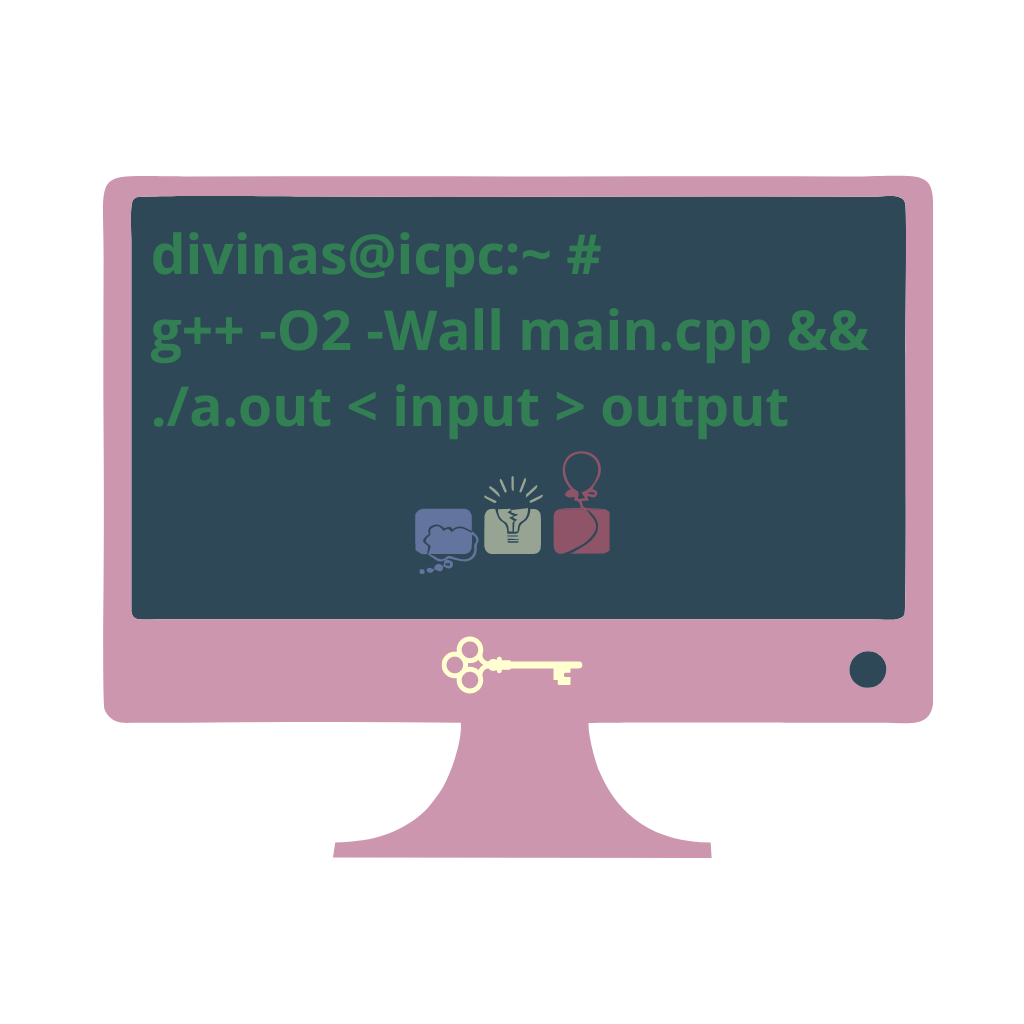
\includegraphics[width=7cm]{icon}\\
    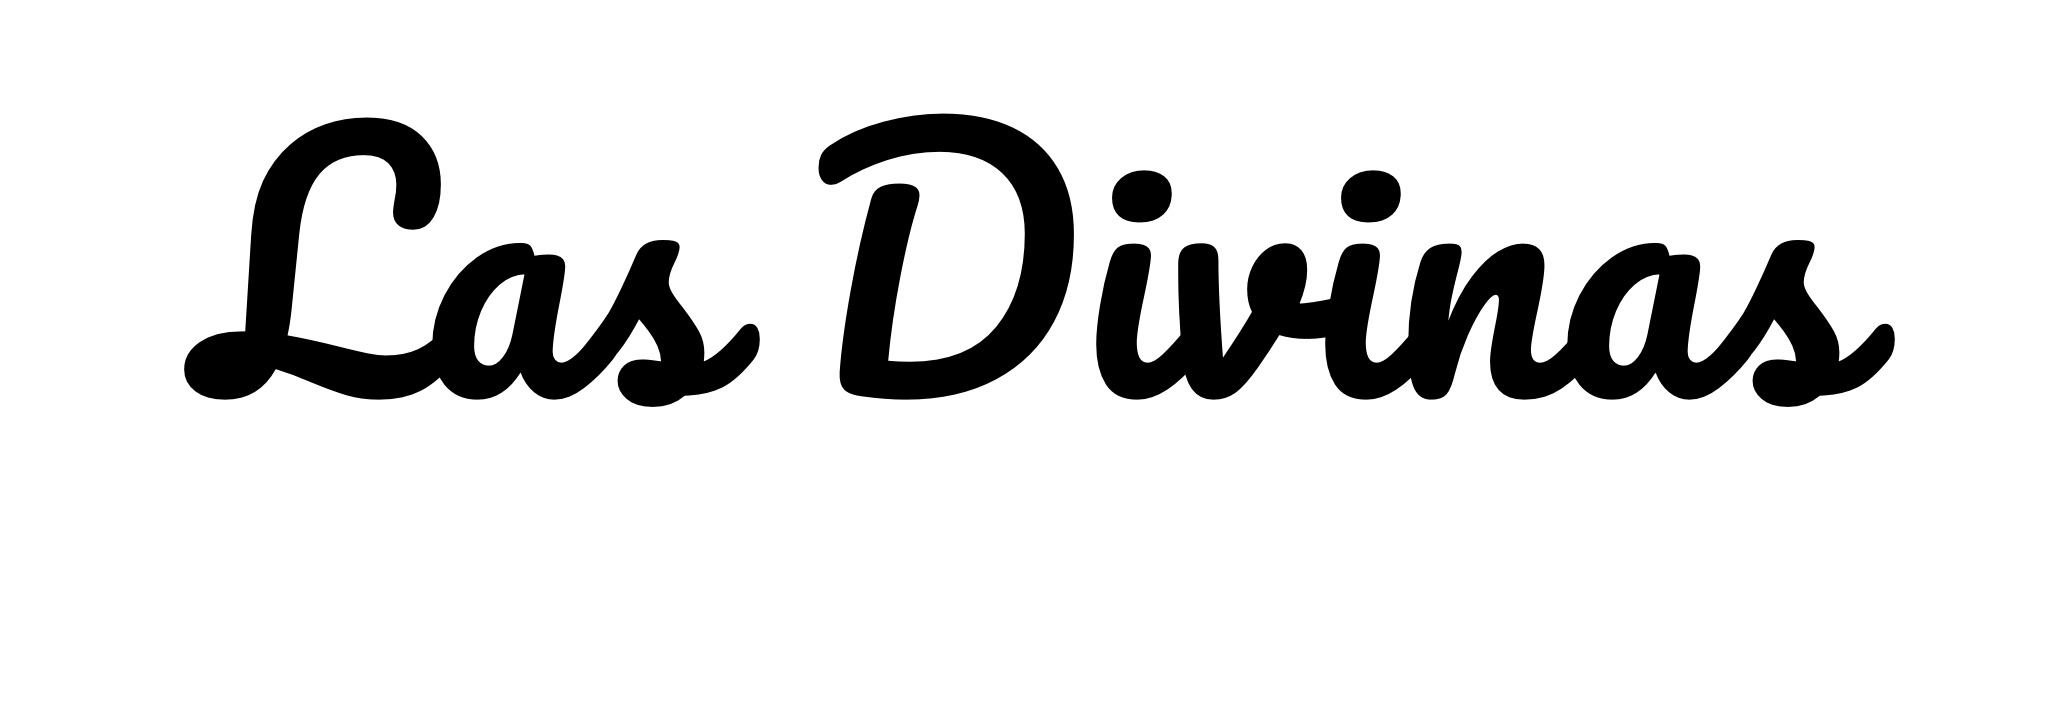
\includegraphics[width=8cm]{logo} % Más fácil que importar la fuente original
    \break
    {\Huge Recopilatorio}\\
    \hfill \break
    \centerline{\rule{7cm}{.4pt}}\\
    \hfill
    \centerline{\rule{7cm}{.4pt}}\\
    \hfill \break
    \hfill \break
    {\LARGE \textbf{Lord\_Friky}}\\
    \hfill \break
    {\LARGE \textbf{valeria-gonzalez}}\\
    \hfill \break
    {\LARGE \textbf{xanemi}}\\
    \hfill \break
    \hfill \break
    \hfill \break
    \hfill \break
    \hfill \break
    \hfill \break
    \hfill \break
    \hfill \break
    \hfill \break
    \hfill \break
    \hfill \break
    \hfill \break
    \hfill \break
    \hfill \break
    \hfill \break
\end{center}

\hfill \break
\hfill \break
\hfill \break
\centerline{{\LARGE Himno}}
\hfill
\centerline{\rule{4cm}{.4pt}}\\
\hfill \break
Nadie pasa de esta esquina\\
Aquí mandan las divinas\\
Porque somos gasolina\\
Gasolina de verdad\\

Todos saben quién manda en este school\\
Porque nosotras somos gente cool\\
Gente que siente, con sangre caliente\\
Que quiere hacerse oír\\

Sea como sea, aquí no entran feas\\
Pa' que lo veas, te voy a mostrar\\
Mira esa fea, aquella otra fea\\
Aquí no pueden entrar\\

Nadie pasa de esta esquina\\
Aquí mandan las divinas\\
Porque somos gasolina\\
Gasolina de verdad\\

Nosotras bailamos bien\\
Dance, dance y mucho dance\\
Lo que pide tu corazón (your heart, your heart)\\
A ti te vamos a dar\\

Las divinas, las divinas, brillan, brillan, como stars\\
Fuera feas, fuera feas, para ustedes no hay lugar\\

Nadie pasa de esta esquina\\
Aquí mandan las divinas\\
Porque somos gasolina\\
Gasolina de verdad\\

Nadie pasa de esta esquina\\
Aquí mandan las divinas\\
Porque somos gasolina\\
Gasolina de verdad\\

Nadie pasa de esta esquina\\
Aquí mandan las divinas\\
Porque somos gasolina\\
Gasolina de verdad\\

Nadie pasa de esta esquina\\
Aquí mandan las divinas\\
Porque somos gasolina\\
Gasolina de verdad\\

Nadie pasa de esta esquina\\
Aquí mandan las divinas\\
Porque somos gasolina\\
Gasolina de verdad\\

\hfill \break
\hfill \break
\hfill \break

\addtocontents{toc}{\setcounter{tocdepth}{1}}
\tableofcontents

\section{Template}
\cppfile{res/template.cpp}

\section{Binary \& Ternary Search}

\subsection{Binary search}
\cppfile{binary_ternary/binary_search.cpp}

\subsection{Binary lifting}
\cppfile{binary_ternary/binary_lifting.cpp}

% To-do: Revisar por qué no quiere funcionar con archivos con acentos.
\subsection{Binary search STL}
\cppfile{binary_ternary/bs_stl.cpp}

\subsection{Ternary search}
\cppfile{binary_ternary/ternary_search.cpp}

\section{Sorting}

\subsection{Merge sort}
\cppfile{sorting/merge_sort.cpp}

% To-do: Agregar quick sort.

\subsection{Sort STL}
\cppfile{sorting/sort_stl.cpp}

\section{Teoría de Números}

\subsection{Criterios de divisivilidad}
\textbf{2:} Último dígito par.\\
\textbf{3:} La suma de los dígitos de x es múltiplo de 3.\\
\textbf{4:} Últimos 2 dígitos son 0 o múltiplo de 4.\\
\textbf{5:} Último dígito 0 ó 5.\\
\textbf{6:} Divisible entre 2 y 3.\\
\textbf{7:} Ayno. Al separar la última cifra de la derecha, multiplicarla por 2 y restarla de las cifras restantes la diferencia es igual a 0 o es un múltiplo de 7.\\
\textbf{8:} Tres últimas cifras divisibles entre 8.\\
\textbf{9:} La suma de los dígitos de x es múltiplo de 9.\\
\textbf{10:} Último dígito 0.\\

\subsection{GCD \& LCM}
\cppfile{number_theory/gcd_lcm.cpp}

\subsection{Cribas}

\subsubsection{Base}
\cppfile{number_theory/cribas/base.cpp}

\subsubsection{Vector de primos}
\cppfile{number_theory/cribas/return_primes.cpp}

\subsubsection{Descomposición factorial}
\cppfile{number_theory/cribas/descomposicion_primos.cpp}

\subsubsection{Criba de mayor divisor}
\cppfile{number_theory/cribas/mayor_divisor.cpp}

\subsubsection{Criba de número de divisores}
\cppfile{number_theory/cribas/numero_divisores.cpp}

\subsubsection{Criba de suma de divisores}
\cppfile{number_theory/cribas/suma_divisores.cpp}

% To-do: Pensar en un mejor nombre para esta clasificación
\section{Estructuras de Datos}

\subsection{Trie}
\cppfile{data_structures/trie.cpp}

\section{Misceláneo}

\subsection{Bitmask}
\cppfile{misc/bitmask.cpp}

\subsection{Depuarador}
\begin{tabularx}{0.5\textwidth} {
    | >{\raggedright\arraybackslash}X 
    | >{\raggedright\arraybackslash}X | }

    \hline
    \multicolumn{2}{|c|}{\textbf{Correr procesos}}\\
    \hline

    \hline
    \multicolumn{1}{|c|}{\textbf{GDB}}
    &
    \multicolumn{1}{c|}{\textbf{LLDB}}\\
    \hline

    % GDB
    \begin{tabular}{@{}p{\linewidth}@{}}
        run <args>\\
        r <args>\\
    \end{tabular}
    & % LLDB
    \begin{tabular}{@{}p{\linewidth}@{}}
        process launch <args>\\
        run <args>\\
        r <args>\\
    \end{tabular}\\
    \hline
\end{tabularx}

\begin{tabularx}{0.5\textwidth} {
    | >{\raggedright\arraybackslash}X 
    | >{\raggedright\arraybackslash}X | }

    \hline
    \multicolumn{2}{|c|}{\textbf{Redirigir IO}}\\
    \hline

    \hline
    \multicolumn{1}{|c|}{\textbf{GDB}}
    &
    \multicolumn{1}{c|}{\textbf{LLDB}}\\
    \hline

    % GDB
    \begin{tabular}{@{}p{\linewidth}@{}}
        run < in\\
        run > out\\
        run < in > out\\
    \end{tabular}
    & % LLDB
    \begin{tabular}{@{}p{\linewidth}@{}}
        settings set target.input-path in\\
        settings set target.output-path out\\
        run\\
    \end{tabular}\\
    \hline
\end{tabularx}

\begin{tabularx}{0.5\textwidth} {
    | >{\raggedright\arraybackslash}X 
    | >{\raggedright\arraybackslash}X | }

    \hline
    \multicolumn{2}{|c|}{\textbf{Argumentos}}\\
    \hline

    \hline
    \multicolumn{1}{|c|}{\textbf{GDB}}
    &
    \multicolumn{1}{c|}{\textbf{LLDB}}\\
    \hline

    % GDB
    \begin{tabular}{@{}p{\linewidth}@{}}
        \textcolor{OliveGreen}{\%} gdb --args a.out 1 2 3\\
        set args 1 2 3\\
        \textcolor{RedOrange}{// Mostrar args}\\
        show args\\
    \end{tabular}
    & % LLDB
    \begin{tabular}{@{}p{\linewidth}@{}}
        \textcolor{OliveGreen}{\%} lldb -- a.out 1 2 3\\
        settings set target.run-args 1 2 3\\
        \textcolor{RedOrange}{// Mostrar args}\\
        settings show target.run-args\\
    \end{tabular}\\
    \hline
\end{tabularx}

\begin{tabularx}{0.5\textwidth} {
    | >{\raggedright\arraybackslash}X 
    | >{\raggedright\arraybackslash}X | }

    \hline
    \multicolumn{2}{|c|}{\textbf{Variables de entorno}}\\
    \hline

    \hline
    \multicolumn{1}{|c|}{\textbf{GDB}}
    &
    \multicolumn{1}{c|}{\textbf{LLDB}}\\
    \hline

    % GDB
    \begin{tabular}{@{}p{\linewidth}@{}}
        set env DEBUG=1\\
        unset env DEBUG\\
    \end{tabular}
    & % LLDB
    \begin{tabular}{@{}p{\linewidth}@{}}
        settings set target.env-vars DEBUG=1\\
        set se target.env-vars DEBUG=1\\
        env DEBUG=1\\
        settings remove target.env-vars DEBUG\\
        set rem target.env-vars DEBUG\\
    \end{tabular}\\
    \hline
\end{tabularx}

\begin{tabularx}{0.5\textwidth} {
    | >{\raggedright\arraybackslash}X 
    | >{\raggedright\arraybackslash}X | }

    \hline
    \multicolumn{2}{|c|}{\textbf{Avanzar}}\\
    \hline

    \hline
    \multicolumn{1}{|c|}{\textbf{GDB}}
    &
    \multicolumn{1}{c|}{\textbf{LLDB}}\\
    \hline

    % GDB
    \begin{tabular}{@{}p{\linewidth}@{}}
        continue\\
        \textcolor{RedOrange}{// Ignorar los siguientes n-1 bp del mismo}\\
        continue n\\
        \textcolor{RedOrange}{// Step in}\\
        step\\
        s\\
        \textcolor{RedOrange}{// Step over}\\
        next\\
        n\\
        \textcolor{RedOrange}{// Step out}\\
        finish\\
        \textcolor{RedOrange}{// Return}\\
        return <RETURN EXPRESSION>\\
    \end{tabular}
    & % LLDB
    \begin{tabular}{@{}p{\linewidth}@{}}
        continue\\
        \textcolor{RedOrange}{// Ignorar los siguientes n bp del mismo}\\
        c -i n\\
        \textcolor{RedOrange}{// Ignorar los siguientes n del x-ésimo bp}\\
        breakpoint modify -i n x
        \textcolor{RedOrange}{// Step in}\\
        thread step-in\\
        step\\
        s\\
        \textcolor{RedOrange}{// Step over}\\
        thread step-over\\
        next\\
        n\\
        \textcolor{RedOrange}{// Step out}\\
        thread step-out\\
        finish\\
        \textcolor{RedOrange}{// Return}\\
        thread return <RETURN EXPRESSION>\\
    \end{tabular}\\
    \hline
\end{tabularx}

\begin{tabularx}{0.5\textwidth} {
    | >{\raggedright\arraybackslash}X 
    | >{\raggedright\arraybackslash}X | }

    \hline
    \multicolumn{2}{|c|}{\textbf{Breakpoints}}\\
    \hline

    \hline
    \multicolumn{1}{|c|}{\textbf{GDB}}
    &
    \multicolumn{1}{c|}{\textbf{LLDB}}\\
    \hline

    % GDB
    \begin{tabular}{@{}p{\linewidth}@{}}
        break main\\
        b test.cpp:12\\
        \textcolor{RedOrange}{// Set bp con condicional}\\
        break foo if n == 43\\
        \textcolor{RedOrange}{// Listar bp}\\
        info break\\
        \textcolor{RedOrange}{// Modificar o quitar la condicional del x-ésimo bp}\\
        cond x <CONDITION>\\
        \textcolor{RedOrange}{// (Des)activar y eliminar bp}\\
        disable x\\
        enable x\\
        delete x\\
    \end{tabular}
    & % LLDB
    \begin{tabular}{@{}p{\linewidth}@{}}
        breakpoint set --name main\\
        br s -f test.cpp -l 12\\
        b test.cpp:12 \textcolor{RedOrange}{// b SÓLO SETEA!!}\\
        \textcolor{RedOrange}{// Set bp con condicional}\\
        br s -n solve -c '(int)n == 43'\\
        \textcolor{RedOrange}{// Listar bp}\\
        breakpoint list\\
        br l\\
        \textcolor{RedOrange}{// Modificar o quitar la condicinal del x-ésimo bp}\\
        br m -c '<CONDITION>' x\\
        \textcolor{RedOrange}{// (Des)activar y eliminar bp}\\
        breakpoint disable x\\
        br en x\\
        br delete x\\
    \end{tabular}\\
    \hline
\end{tabularx}

\begin{tabularx}{0.5\textwidth} {
    | >{\raggedright\arraybackslash}X 
    | >{\raggedright\arraybackslash}X | }

    \hline
    \multicolumn{2}{|c|}{\textbf{Watchpoints}}\\
    \hline

    \hline
    \multicolumn{1}{|c|}{\textbf{GDB}}
    &
    \multicolumn{1}{c|}{\textbf{LLDB}}\\
    \hline

    % GDB
    \begin{tabular}{@{}p{\linewidth}@{}}
        break main\\
        b test.cpp:12\\
        \textcolor{RedOrange}{// Set bp con condicional}\\
        break foo if n == 43\\
        \textcolor{RedOrange}{// Listar bp}\\
        info break\\
        \textcolor{RedOrange}{// Modificar o quitar la condicional del x-ésimo bp}\\
        cond x <CONDITION>\\
        \textcolor{RedOrange}{// (Des)activar y eliminar bp}\\
        disable x\\
        enable x\\
        delete x\\
    \end{tabular}
    & % LLDB
    \begin{tabular}{@{}p{\linewidth}@{}}
        breakpoint set --name main\\
        br s -f test.cpp -l 12\\
        b test.cpp:12 \textcolor{RedOrange}{// b SÓLO SETEA!!}\\
        \textcolor{RedOrange}{// Set bp con condicional}\\
        br s -n solve -c '(int)n == 43'\\
        \textcolor{RedOrange}{// Listar bp}\\
        breakpoint list\\
        br l\\
        \textcolor{RedOrange}{// Modificar o quitar la condicinal del x-ésimo bp}\\
        br m -c '<CONDITION>' x\\
        \textcolor{RedOrange}{// (Des)activar y eliminar bp}\\
        breakpoint disable x\\
        br en x\\
        br delete x\\
    \end{tabular}\\
    \hline
\end{tabularx}

\end{document}
